% Created by tikzDevice version 0.12.3.1 on 2021-12-16 22:51:57
% !TEX encoding = UTF-8 Unicode
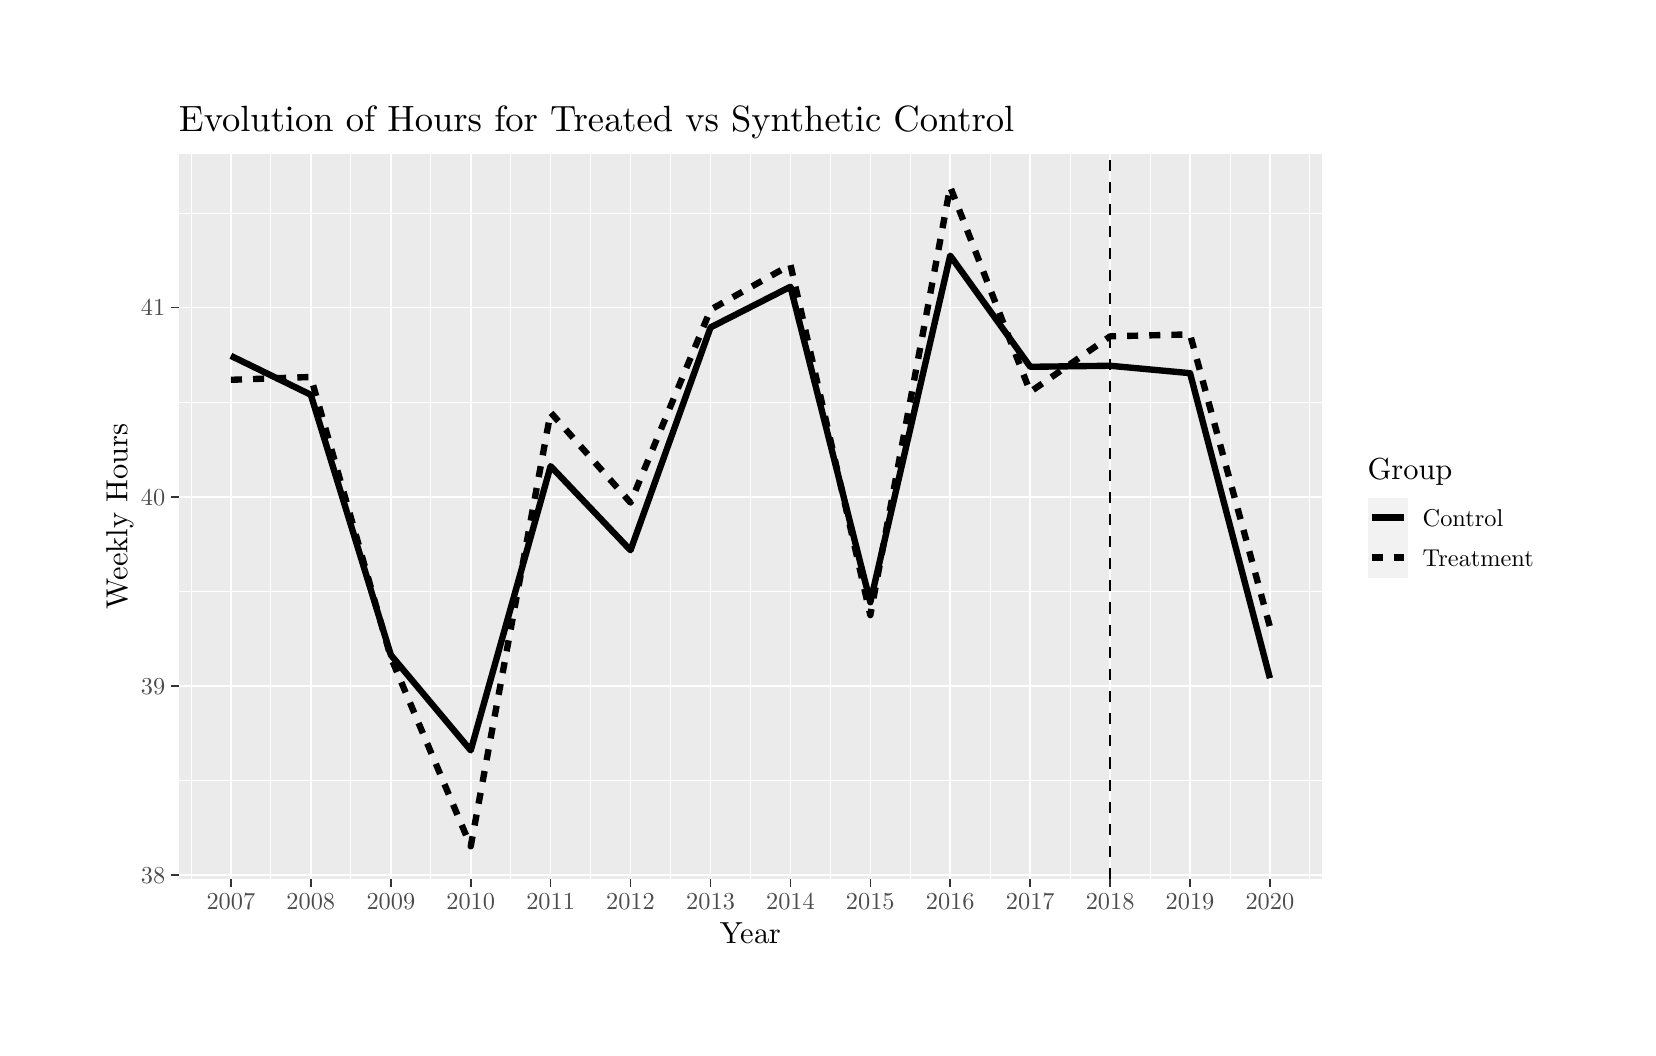
\begin{tikzpicture}[x=1pt,y=1pt]
\definecolor{fillColor}{RGB}{255,255,255}
\path[use as bounding box,fill=fillColor,fill opacity=0.00] (0,0) rectangle (578.16,361.35);
\begin{scope}
\path[clip] (  0.00,  0.00) rectangle (578.16,361.35);
\definecolor{drawColor}{RGB}{255,255,255}
\definecolor{fillColor}{RGB}{255,255,255}

\path[draw=drawColor,line width= 0.6pt,line join=round,line cap=round,fill=fillColor] (  0.00,  0.00) rectangle (578.16,361.35);
\end{scope}
\begin{scope}
\path[clip] ( 54.66, 53.64) rectangle (467.65,315.74);
\definecolor{fillColor}{gray}{0.92}

\path[fill=fillColor] ( 54.66, 53.64) rectangle (467.65,315.74);
\definecolor{drawColor}{RGB}{255,255,255}

\path[draw=drawColor,line width= 0.3pt,line join=round] ( 54.66, 89.25) --
	(467.65, 89.25);

\path[draw=drawColor,line width= 0.3pt,line join=round] ( 54.66,157.63) --
	(467.65,157.63);

\path[draw=drawColor,line width= 0.3pt,line join=round] ( 54.66,226.01) --
	(467.65,226.01);

\path[draw=drawColor,line width= 0.3pt,line join=round] ( 54.66,294.39) --
	(467.65,294.39);

\path[draw=drawColor,line width= 0.3pt,line join=round] ( 59.01, 53.64) --
	( 59.01,315.74);

\path[draw=drawColor,line width= 0.3pt,line join=round] ( 87.87, 53.64) --
	( 87.87,315.74);

\path[draw=drawColor,line width= 0.3pt,line join=round] (116.77, 53.64) --
	(116.77,315.74);

\path[draw=drawColor,line width= 0.3pt,line join=round] (145.67, 53.64) --
	(145.67,315.74);

\path[draw=drawColor,line width= 0.3pt,line join=round] (174.53, 53.64) --
	(174.53,315.74);

\path[draw=drawColor,line width= 0.3pt,line join=round] (203.39, 53.64) --
	(203.39,315.74);

\path[draw=drawColor,line width= 0.3pt,line join=round] (232.30, 53.64) --
	(232.30,315.74);

\path[draw=drawColor,line width= 0.3pt,line join=round] (261.20, 53.64) --
	(261.20,315.74);

\path[draw=drawColor,line width= 0.3pt,line join=round] (290.06, 53.64) --
	(290.06,315.74);

\path[draw=drawColor,line width= 0.3pt,line join=round] (318.92, 53.64) --
	(318.92,315.74);

\path[draw=drawColor,line width= 0.3pt,line join=round] (347.82, 53.64) --
	(347.82,315.74);

\path[draw=drawColor,line width= 0.3pt,line join=round] (376.72, 53.64) --
	(376.72,315.74);

\path[draw=drawColor,line width= 0.3pt,line join=round] (405.58, 53.64) --
	(405.58,315.74);

\path[draw=drawColor,line width= 0.3pt,line join=round] (434.45, 53.64) --
	(434.45,315.74);

\path[draw=drawColor,line width= 0.3pt,line join=round] (463.31, 53.64) --
	(463.31,315.74);

\path[draw=drawColor,line width= 0.6pt,line join=round] ( 54.66, 55.05) --
	(467.65, 55.05);

\path[draw=drawColor,line width= 0.6pt,line join=round] ( 54.66,123.44) --
	(467.65,123.44);

\path[draw=drawColor,line width= 0.6pt,line join=round] ( 54.66,191.82) --
	(467.65,191.82);

\path[draw=drawColor,line width= 0.6pt,line join=round] ( 54.66,260.20) --
	(467.65,260.20);

\path[draw=drawColor,line width= 0.6pt,line join=round] ( 73.44, 53.64) --
	( 73.44,315.74);

\path[draw=drawColor,line width= 0.6pt,line join=round] (102.30, 53.64) --
	(102.30,315.74);

\path[draw=drawColor,line width= 0.6pt,line join=round] (131.24, 53.64) --
	(131.24,315.74);

\path[draw=drawColor,line width= 0.6pt,line join=round] (160.10, 53.64) --
	(160.10,315.74);

\path[draw=drawColor,line width= 0.6pt,line join=round] (188.96, 53.64) --
	(188.96,315.74);

\path[draw=drawColor,line width= 0.6pt,line join=round] (217.83, 53.64) --
	(217.83,315.74);

\path[draw=drawColor,line width= 0.6pt,line join=round] (246.77, 53.64) --
	(246.77,315.74);

\path[draw=drawColor,line width= 0.6pt,line join=round] (275.63, 53.64) --
	(275.63,315.74);

\path[draw=drawColor,line width= 0.6pt,line join=round] (304.49, 53.64) --
	(304.49,315.74);

\path[draw=drawColor,line width= 0.6pt,line join=round] (333.35, 53.64) --
	(333.35,315.74);

\path[draw=drawColor,line width= 0.6pt,line join=round] (362.29, 53.64) --
	(362.29,315.74);

\path[draw=drawColor,line width= 0.6pt,line join=round] (391.15, 53.64) --
	(391.15,315.74);

\path[draw=drawColor,line width= 0.6pt,line join=round] (420.02, 53.64) --
	(420.02,315.74);

\path[draw=drawColor,line width= 0.6pt,line join=round] (448.88, 53.64) --
	(448.88,315.74);
\definecolor{drawColor}{RGB}{0,0,0}

\path[draw=drawColor,line width= 2.3pt,dash pattern=on 4pt off 4pt ,line join=round] ( 73.44,234.10) --
	(102.30,235.12) --
	(131.24,133.73) --
	(160.10, 65.55) --
	(188.96,222.32) --
	(217.83,189.72) --
	(246.77,259.46) --
	(275.63,275.65) --
	(304.49,149.06) --
	(333.35,303.83) --
	(362.29,229.74) --
	(391.15,249.81) --
	(420.02,250.52) --
	(448.88,144.86);

\path[draw=drawColor,line width= 2.3pt,line join=round] ( 73.44,242.76) --
	(102.30,228.71) --
	(131.24,134.66) --
	(160.10,100.19) --
	(188.96,202.91) --
	(217.83,172.51) --
	(246.77,253.05) --
	(275.63,267.74) --
	(304.49,153.73) --
	(333.35,278.99) --
	(362.29,238.80) --
	(391.15,239.18) --
	(420.02,236.50) --
	(448.88,126.28);

\path[draw=drawColor,line width= 0.6pt,dash pattern=on 4pt off 4pt ,line join=round] (391.15, 53.64) -- (391.15,315.74);
\end{scope}
\begin{scope}
\path[clip] (  0.00,  0.00) rectangle (578.16,361.35);
\definecolor{drawColor}{gray}{0.30}

\node[text=drawColor,anchor=base east,inner sep=0pt, outer sep=0pt, scale=  0.88] at ( 49.71, 52.02) {38};

\node[text=drawColor,anchor=base east,inner sep=0pt, outer sep=0pt, scale=  0.88] at ( 49.71,120.41) {39};

\node[text=drawColor,anchor=base east,inner sep=0pt, outer sep=0pt, scale=  0.88] at ( 49.71,188.79) {40};

\node[text=drawColor,anchor=base east,inner sep=0pt, outer sep=0pt, scale=  0.88] at ( 49.71,257.17) {41};
\end{scope}
\begin{scope}
\path[clip] (  0.00,  0.00) rectangle (578.16,361.35);
\definecolor{drawColor}{gray}{0.20}

\path[draw=drawColor,line width= 0.6pt,line join=round] ( 51.91, 55.05) --
	( 54.66, 55.05);

\path[draw=drawColor,line width= 0.6pt,line join=round] ( 51.91,123.44) --
	( 54.66,123.44);

\path[draw=drawColor,line width= 0.6pt,line join=round] ( 51.91,191.82) --
	( 54.66,191.82);

\path[draw=drawColor,line width= 0.6pt,line join=round] ( 51.91,260.20) --
	( 54.66,260.20);
\end{scope}
\begin{scope}
\path[clip] (  0.00,  0.00) rectangle (578.16,361.35);
\definecolor{drawColor}{gray}{0.20}

\path[draw=drawColor,line width= 0.6pt,line join=round] ( 73.44, 50.89) --
	( 73.44, 53.64);

\path[draw=drawColor,line width= 0.6pt,line join=round] (102.30, 50.89) --
	(102.30, 53.64);

\path[draw=drawColor,line width= 0.6pt,line join=round] (131.24, 50.89) --
	(131.24, 53.64);

\path[draw=drawColor,line width= 0.6pt,line join=round] (160.10, 50.89) --
	(160.10, 53.64);

\path[draw=drawColor,line width= 0.6pt,line join=round] (188.96, 50.89) --
	(188.96, 53.64);

\path[draw=drawColor,line width= 0.6pt,line join=round] (217.83, 50.89) --
	(217.83, 53.64);

\path[draw=drawColor,line width= 0.6pt,line join=round] (246.77, 50.89) --
	(246.77, 53.64);

\path[draw=drawColor,line width= 0.6pt,line join=round] (275.63, 50.89) --
	(275.63, 53.64);

\path[draw=drawColor,line width= 0.6pt,line join=round] (304.49, 50.89) --
	(304.49, 53.64);

\path[draw=drawColor,line width= 0.6pt,line join=round] (333.35, 50.89) --
	(333.35, 53.64);

\path[draw=drawColor,line width= 0.6pt,line join=round] (362.29, 50.89) --
	(362.29, 53.64);

\path[draw=drawColor,line width= 0.6pt,line join=round] (391.15, 50.89) --
	(391.15, 53.64);

\path[draw=drawColor,line width= 0.6pt,line join=round] (420.02, 50.89) --
	(420.02, 53.64);

\path[draw=drawColor,line width= 0.6pt,line join=round] (448.88, 50.89) --
	(448.88, 53.64);
\end{scope}
\begin{scope}
\path[clip] (  0.00,  0.00) rectangle (578.16,361.35);
\definecolor{drawColor}{gray}{0.30}

\node[text=drawColor,anchor=base,inner sep=0pt, outer sep=0pt, scale=  0.88] at ( 73.44, 42.63) {2007};

\node[text=drawColor,anchor=base,inner sep=0pt, outer sep=0pt, scale=  0.88] at (102.30, 42.63) {2008};

\node[text=drawColor,anchor=base,inner sep=0pt, outer sep=0pt, scale=  0.88] at (131.24, 42.63) {2009};

\node[text=drawColor,anchor=base,inner sep=0pt, outer sep=0pt, scale=  0.88] at (160.10, 42.63) {2010};

\node[text=drawColor,anchor=base,inner sep=0pt, outer sep=0pt, scale=  0.88] at (188.96, 42.63) {2011};

\node[text=drawColor,anchor=base,inner sep=0pt, outer sep=0pt, scale=  0.88] at (217.83, 42.63) {2012};

\node[text=drawColor,anchor=base,inner sep=0pt, outer sep=0pt, scale=  0.88] at (246.77, 42.63) {2013};

\node[text=drawColor,anchor=base,inner sep=0pt, outer sep=0pt, scale=  0.88] at (275.63, 42.63) {2014};

\node[text=drawColor,anchor=base,inner sep=0pt, outer sep=0pt, scale=  0.88] at (304.49, 42.63) {2015};

\node[text=drawColor,anchor=base,inner sep=0pt, outer sep=0pt, scale=  0.88] at (333.35, 42.63) {2016};

\node[text=drawColor,anchor=base,inner sep=0pt, outer sep=0pt, scale=  0.88] at (362.29, 42.63) {2017};

\node[text=drawColor,anchor=base,inner sep=0pt, outer sep=0pt, scale=  0.88] at (391.15, 42.63) {2018};

\node[text=drawColor,anchor=base,inner sep=0pt, outer sep=0pt, scale=  0.88] at (420.02, 42.63) {2019};

\node[text=drawColor,anchor=base,inner sep=0pt, outer sep=0pt, scale=  0.88] at (448.88, 42.63) {2020};
\end{scope}
\begin{scope}
\path[clip] (  0.00,  0.00) rectangle (578.16,361.35);
\definecolor{drawColor}{RGB}{0,0,0}

\node[text=drawColor,anchor=base,inner sep=0pt, outer sep=0pt, scale=  1.10] at (261.16, 30.59) {Year};
\end{scope}
\begin{scope}
\path[clip] (  0.00,  0.00) rectangle (578.16,361.35);
\definecolor{drawColor}{RGB}{0,0,0}

\node[text=drawColor,rotate= 90.00,anchor=base,inner sep=0pt, outer sep=0pt, scale=  1.10] at ( 36.03,184.69) {Weekly Hours};
\end{scope}
\begin{scope}
\path[clip] (  0.00,  0.00) rectangle (578.16,361.35);
\definecolor{fillColor}{RGB}{255,255,255}

\path[fill=fillColor] (478.65,157.13) rectangle (549.71,212.25);
\end{scope}
\begin{scope}
\path[clip] (  0.00,  0.00) rectangle (578.16,361.35);
\definecolor{drawColor}{RGB}{0,0,0}

\node[text=drawColor,anchor=base west,inner sep=0pt, outer sep=0pt, scale=  1.10] at (484.15,198.11) {Group};
\end{scope}
\begin{scope}
\path[clip] (  0.00,  0.00) rectangle (578.16,361.35);
\definecolor{fillColor}{gray}{0.95}

\path[fill=fillColor] (484.15,177.08) rectangle (498.60,191.54);
\end{scope}
\begin{scope}
\path[clip] (  0.00,  0.00) rectangle (578.16,361.35);
\definecolor{drawColor}{RGB}{0,0,0}

\path[draw=drawColor,line width= 2.3pt,line join=round] (485.59,184.31) -- (497.16,184.31);
\end{scope}
\begin{scope}
\path[clip] (  0.00,  0.00) rectangle (578.16,361.35);
\definecolor{drawColor}{RGB}{0,0,0}

\path[draw=drawColor,line width= 2.3pt,line join=round] (485.59,184.31) -- (497.16,184.31);
\end{scope}
\begin{scope}
\path[clip] (  0.00,  0.00) rectangle (578.16,361.35);
\definecolor{fillColor}{gray}{0.95}

\path[fill=fillColor] (484.15,162.63) rectangle (498.60,177.08);
\end{scope}
\begin{scope}
\path[clip] (  0.00,  0.00) rectangle (578.16,361.35);
\definecolor{drawColor}{RGB}{0,0,0}

\path[draw=drawColor,line width= 2.3pt,dash pattern=on 4pt off 4pt ,line join=round] (485.59,169.86) -- (497.16,169.86);
\end{scope}
\begin{scope}
\path[clip] (  0.00,  0.00) rectangle (578.16,361.35);
\definecolor{drawColor}{RGB}{0,0,0}

\path[draw=drawColor,line width= 2.3pt,dash pattern=on 4pt off 4pt ,line join=round] (485.59,169.86) -- (497.16,169.86);
\end{scope}
\begin{scope}
\path[clip] (  0.00,  0.00) rectangle (578.16,361.35);
\definecolor{drawColor}{RGB}{0,0,0}

\node[text=drawColor,anchor=base west,inner sep=0pt, outer sep=0pt, scale=  0.88] at (504.10,181.28) {Control};
\end{scope}
\begin{scope}
\path[clip] (  0.00,  0.00) rectangle (578.16,361.35);
\definecolor{drawColor}{RGB}{0,0,0}

\node[text=drawColor,anchor=base west,inner sep=0pt, outer sep=0pt, scale=  0.88] at (504.10,166.82) {Treatment};
\end{scope}
\begin{scope}
\path[clip] (  0.00,  0.00) rectangle (578.16,361.35);
\definecolor{drawColor}{RGB}{0,0,0}

\node[text=drawColor,anchor=base west,inner sep=0pt, outer sep=0pt, scale=  1.32] at ( 54.66,323.81) {Evolution of Hours for Treated vs Synthetic Control};
\end{scope}
\end{tikzpicture}
